\subsection{First Experience}

\subsubsection{Capturing packets from an execution of traceroute}
wasa

\subsubsection{Basic IPv4}
wasa

\subsubsection{Fragmentation}

This section of the experience was done on a Windows machine, and so we had to
work with the downloaded trace file.

First, we looked for the first IP datagram containing the first part of the
segment sent to the server. After finding it (it wasn't the first packet), we
looked for any field that might indicate that it was fragmented.

\begin{figure}[htbp]
    \centering
    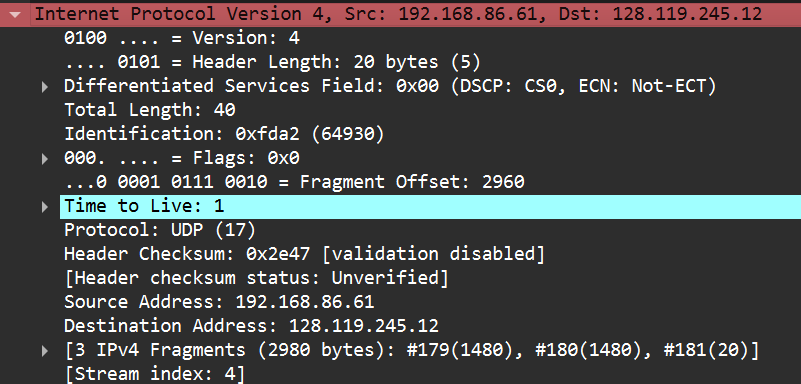
\includegraphics[width=1\linewidth]{img/2/1.png}
    \caption{Packet IP header}\label{fig:2_1}
\end{figure}

We can see that there's a field containing 3 IPv4 fragments, and thus we can
conclude that it was indeed fragmented.

We then wanted to know if this packet was the first fragment, or a latter one.
Seeing that the \textbf{fragment offset} value is nonzero, we can conclude that
this is a latter fragment.

The total number of bytes in this datagram (payload plus header) is 2972 plus
20, i.e. 2992.